%!TEX root = ../dokumentation.tex

% -------------------------------
\chapter{Literature and State of the Art} % ~5–6 pages, ~2000–2400 words
% -------------------------------
\label{chap:literature}
In this chapter, the current state of the art and literature get presented.
First, the development of machine learning to distributed machine learning gets sketched. Then, \ac{ASTRA-Sim} gets presented and compared to alternative \ac{DML} (simulation) approaches.
Lastly, \ac{UI} and \ac{UX} best practices, with a focus on evaluation criteria and \aac{UI} for scientific tools get presented. 

\section{Development of Distributed Machine Learning}
% 1. ML: Zyklus, Purpose
\ac{DML} is a concept based on \ac{ML} distributed on multiple machines. To deeply understand it, one needs to know basics of \ac{ML} first.

\subsubsection*{History of Machine Learning}
%% Historical
%%% Early Turing + (59er book)
The concept of machines learning similar to human learning was first proposed in 1950 by Turing \cite{turing_computing_1989}. He proposed the first known of theoretical description of the concept that later became known as \ac{AI}.
In his paper, he introduces basics such as the idea that machines could simulate human intelligence, if they are given the right data and algorithms. He states that learning, similar to children education is central and supports it with evolutionary algorithms. He claims that machines, which can be seen as discrete-state machines, can simulate anything, which enables them to universal computational capabilities useable for \ac{ML}.

Following this basic idea, the first working \ac{ML} program was introduced in 1959 by Samuel \cite{samuel_studies_1959}. Samuel presents a program that is able to play the game checkers better than its programmer, with only 8 -- 10 hours of playing and information such as rules of the game. This program is based on self-improvement, it adjusts its strategy based on previous outcomes. Therefor it is the first documented ``self learning'' algorithm. The learn process has two approaches; one is memorizing each board positions evaluation and the other one to adjust this evaluation function based on experiences.  In this version, it uses the delta between expected and actual result to update expected parameters.

%%% Statistical Learning
At this time early \ac{ML} begun and these concepts were expanded, as in 1963 Abramson presents further pattern recognition and machine learning approaches \cite{abramson_pattern_1963}. Here, statistical approaches were introduced and data was first viewed as vectors in a multidimensional space. He framed pattern recognition as a classification problem in vector spaces with two subproblems, being the partitioning techniques and choice of measurements. 
Also, the first idea of a distinction between supervised and unsupervised training was explained. But there were still gaps in research that only had to be discovered in the following years, like the selection of relevant features.

In the following years, many concepts of \ac{ML} were revised and newly discovered. Such as backpropagation in the 80s \cite{rojas_backpropagation_1996}, that introduced using gradient calculation for loss correction, or the big data field especially in the 2000s \cite{perez_karich_emergence_2025}. 

%% Reason for Distribution
As \ac{ML} grew and gained importance, problems regarding growing demands arose. One is the growing availability of datasets. With more data available, training once possible in a few ours might take days or even years to finish, if not optimized. The data is also more complex, forming vectors of increasing dimensions, compared to past data.
Also, models are increasing in complexity, so do deep networks have trillions of parameters compared to shallow neural networks in 1990 \cite{oneto_limitations_2020}.
These problems demand a solution. Parts of these problems could be solved by scaling with improved hardware as an option, as chips could be made more efficient by scaling with smaller transistors~\cite{sevilla_compute_2022}. This approach, based on Moore's law~\cite{moore_cramming_2006}, is not upholdable anymore, in the 2010s it was declared ``dead''~\cite{theis_end_2017}.
% This approach, based on Moore's law, is not upholdable anymore, in 2022 it was declared ``dead'' by Nvidias CEO~\cite{.}.
Naturally, the developed solution was distributing the training. \ac{DML} is a subset of \ac{ML} that splits the training process onto multiple \acp{NPU}~\cite{bekkerman_scaling_2011}.
In 2024, distributed training became the standard for large scale systems and remained the state of the art~\cite{li_understanding_2024}. 

\subsubsection*{DML Characteristics}
%% Either topic separated or timeline
%% Clusters, GPUs/TPUs, cloud computing, IaaS (SimGrid IaaS paper can illustrate system-level concerns). computation
%% Topologies
With \ac{DML} a solution for scaling was introduced, and new challenges have to be solved.
Distributing the machine learning process is not straightforward---it depends on many factors, such as the way of splitting, network latencies and communication strategies.

% TODO describe very basic the basics like computation & communciation
The basic \ac{DML} process combines individual computation of different workers with a communication between them. That way they can train one model together by separating tasks. This separation can follow two approaches visualized in figure \ref{fig:parallelism} by the official PyTorch website (https://docs.pytorch.org/torchrec/high-level-arch.html) \cite{noauthor_torchrec_nodate}. % Torchrec SOURCE
One, called data parallelism, is splitting the data that the model is supposed to train on. That way, all workers iteratively train a part of the data onto the same model and communicate the models parameters and gradients between computation iterations. 
While data parallelism has the advantage of being easily implementable and reduce computation times nearly linearly (TODO check if true lol), its communication can create new overheads if workloads are distributed unevenly and a synchronous communication is used. Detailed on that and further advantages and disadvantages get discussed in section \ref{sec:discussion}.
The other parallelization, called model parallelism, a type being for example pipeline parallelism, is focussing on splitting the models parts onto the workers. Here, the layers of the model are divided and trained separately with according communication. This has the advantage of enabling training to include large models, but requires more complicated communication than data parallelism.
Common are also hybrid approaches in which both data and models get split. This combines advantages such as a high scalability and the possibility for an efficient training performance, but new introduced challenges are finding the optimal distribution  between data and model parallel strategies as well as for load balancing communication and computation efficiently~\cite{boehm_hybrid_2014}.

\begin{figure}[h]  % TODO make an own visualization, and maybe use H instead
  \centering
  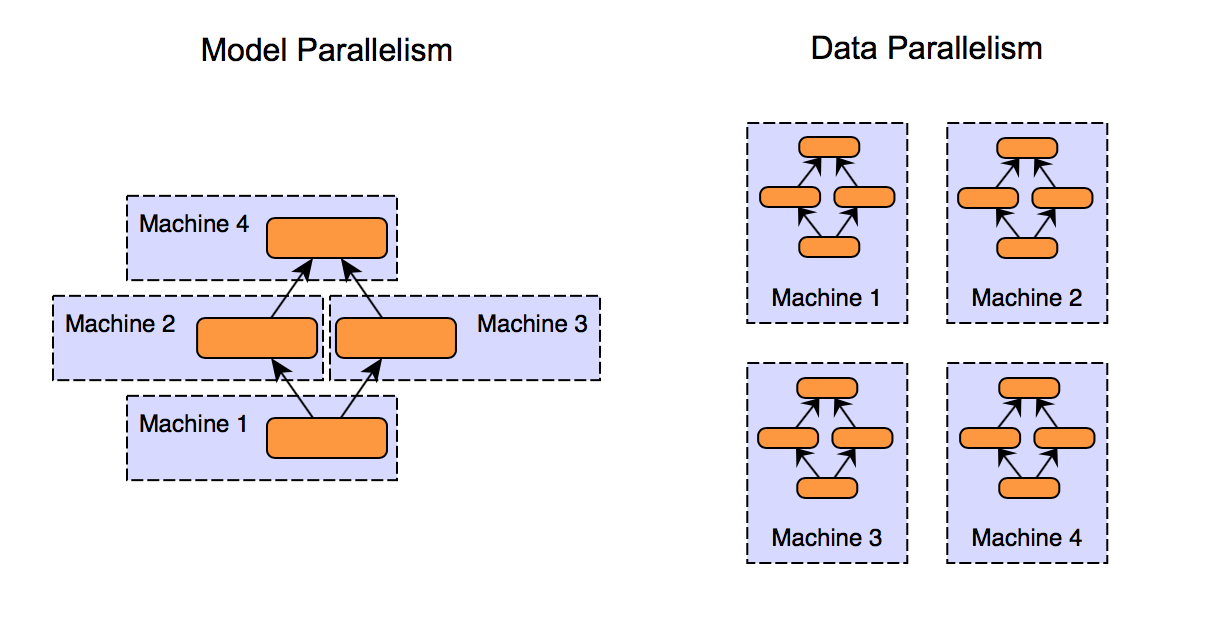
\includegraphics[width=0.7\linewidth]{parallelism.png}
  \caption{Parallelism Strategies}
  \label{fig:parallelism}
\end{figure}

% 2. Hardware: Topologies, latency, bandwith, structure
\subsubsection*{Hardware Details}
The workers used in the \ac{DML} process, generally called \acp{NPU}, are usually \acp{GPU}. They can appear in high amounts, from 8 \acp{GPU} for research purposes to 1000s for \acp{LLM} like GPT-5~\cite{network_how_2024}. % SOURCE

A set of \acp{NPU} structured together is called cluster, and each cluster is able to take different amounts of them. How they are connected in each cluster is described by a physical network topology. Every cluster in one machine, or called node, respectively, communicates via intra-node-communication. \acp{NPU} communicating between different nodes is possible over \acp{NIC}, which are connected in an inter-node-network.
% Bandwidths and Latencies
While intra-node communication has low latencies and high bandwidths, due to connections via NVLinks or PCIle switches, inter-node-communication has rater high latencies and low bandwidths beacause of used network interfaces like InfiniBand~\cite{gangidi_rdma_2024}. % source sais: Intra-node communication is generally faster due to high-bandwidth NVLink or PCIe connections, whereas inter-node communication relies on slower network interfaces such as InfiniBand.
This would make a distributed training with few machines attractive, but realistic distribution onto many machines is much more scalable.
That is due to the limited amount of \acp{GPU} in one server. % TODO check source first: A Study on Distributed Strategies for Deep Learning Applications in GPU Clusters; source: While training on fewer nodes reduces communication overhead, it limits the total number of GPUs available. For large models, scaling across many nodes becomes necessary despite the increased communication cost.
Therefore, large distributed systems use and depend on both, intra and inter-node-communication.
% Topologies
The topologies of distributed systems can be based on different architectures. Verbreaken presents that there are four types of topologies that can exist for distributed systems~\cite{verbraeken_survey_2020}. Generally they can be divided into centralized, decentralized and fully distributed topologies, based on the degree of the distribution. A structural overview can be found in~\ref{fig:topologies}.

% have a central server that orchestrates them or be decentralized instead. .

\begin{figure}[H]  % TODO make a better visualization, especially for the parameter server
  \centering
  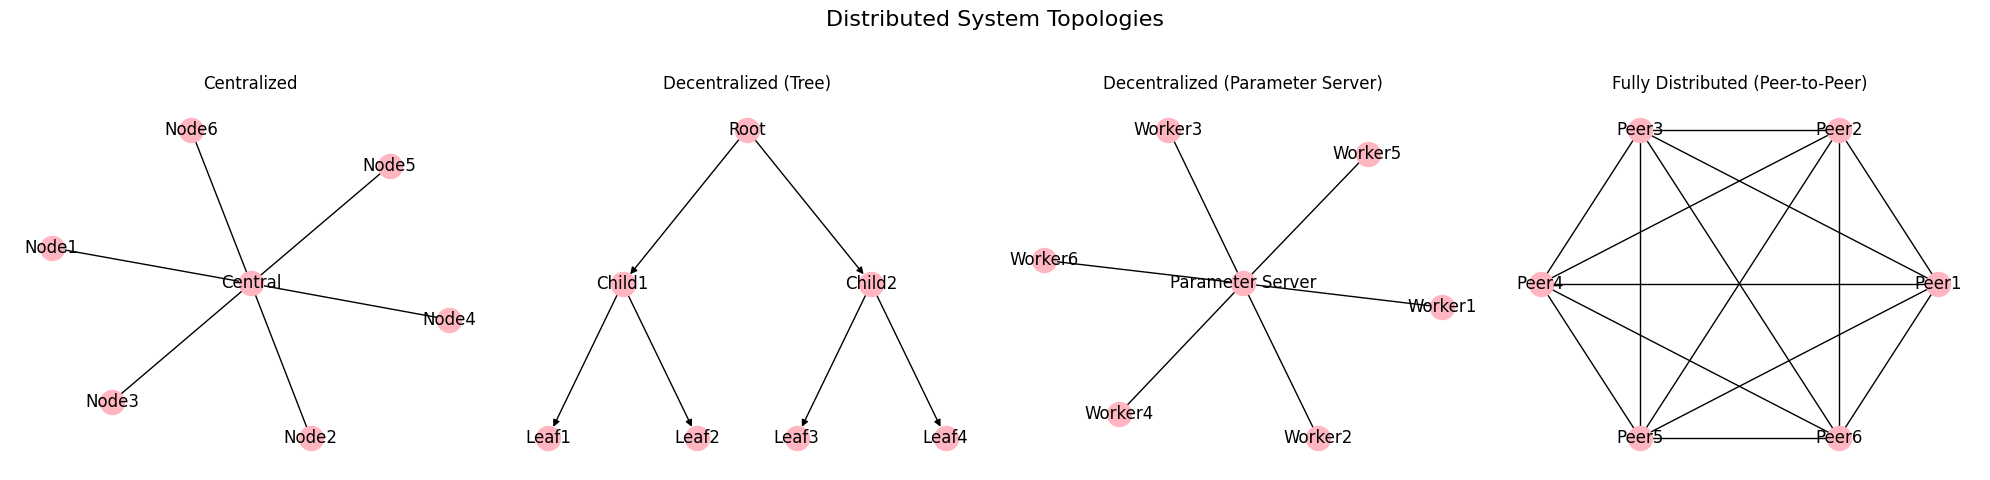
\includegraphics[width=1\linewidth]{topologies.png}
  \caption{Network Topologies}
  \label{fig:topologies}
\end{figure}

The centralized topology is characterized by a strict hierarchical structure in which all nodes are connected with one central server that orchestrates them and performs the necessary steps for the combination of the machine learning. It serves a simple coordination but is limited in scalability due to having a single point of failure.

The tree topology is a decentralized topology in which the nodes are structured hierarchical. The communication takes place between the nodes in specific directions. Information is communicated upwards and distributed downwards. This is scalable as every node only communicates with children or parents.

The parameter server topology is a second decentralized topology that combines centralized parameter servers to store and retrieve gradients with decentralized \ac{ML} nodes. These servers have a shared memory, so the parameters can be synchronized between multiple parts. The disadvantage of this is that all communication happens at the parameter servers, creating bottlenecks if many workers are combined with few servers.

A fully distributed topology works like a peer-to-peer network, meaning each node holds its own copy of the models parameters and is able to communicate with all other nodes. Communication is possible in every direction and at any time. This is very scalable, as new workers can be added without a high centralized overload, but it has the disadvantage that the communication can create a high overhead if every worker broadcasts its information.

Topologies can be asymmetric or symmetric, depending on if the connections are bidirectional or unidirectional. For fully distributed systems both could be possible, while all other topologies depend on bidirectional connections~\cite{won_tacos_2024}.

% TODO check if something hardware related is missing
% TODO add common hardware solutions such as NVLink etc

% Different System architectures can be used. For example an all to all approach in which all 
% - synchronization: when communication happens
% - 
% needs a split of the process, by model or data and new limiting factors are network communications. 


\subsubsection*{Communication Strategies}
%% Parallelization strategies: data vs model parallelism, parameter servers, federated learning.

While physical topologies are showing different ways of organizing and centralizing the connections of machines, logical topologies can be used to specify how the actual communication is practiced.  
For this two main communication strategies a distinction between two new types of parallelization has to be made. They can either be synchronous, meaning all machines communicate at the same time collaboratively, or asynchronous, where each worker communicates as soon as it is finished with its own computation. Both are not applicable to every physical topology. Asynchronous communication is best suited for decentralized topologies with parameter servers. In that case workers push and pull parameters anytime necessary without the need for waiting for other workers to finish.
Possible are also more varying approaches such as a trade-off version, called local \ac{SGD}, that allows workers to communicate asynchronous for a set amount of time until needing to synchronize \cite{verbraeken_survey_2020} or \ac{SSP}, which additionally allows for cached parameters to be used for synchronization for the set amount of time~\cite{tang_communication-efficient_2023}. 

% 3. communication: topologies, collectives, synchronization (also system architectures such as gossip?)
Depending on the parallelization strategies and split of the training process varying types of communication have to be performed. 
While data parallelism relies on frequent exchange of calculated gradients, for example tensor parallelism, a type of model parallelism, needs to communicate between steps as early as in the forward pass \cite{dong_towards_2024}. % TODO explain forward pass bevore too

%% Collectives
Those types of communications can be achieved by using for example communication collectives. That are a set of synchronized communication patterns, which can be used for sharing and combining information across multiple machines in distributed systems, for instance \textit{All-Reduce}, \textit{All-to-All} or \textit{Reduce-Scatter}. 
These collectives are most common for data parallelism, as they help to synchronize and combine gradients, and share parameters. They are blocking, meaning, nodes have to wait for each other's computation to finish, and they have to be orchestrated by a centralized controller.
Generally, collectives can be separated into redistributive operations, that share data and consolidative operations, that aggregate data. 
The most common collective used for data parallelism is \textit{All-Reduce}. In the following the approach of collectives is explained, based on \textit{All-Reduce} as an example. For guidance, figure \ref{fig:collectives} shows a visualization of the collective.
The source for this explanation is the $25$th course lecture of UC Berkeley's course \textit{CS 168} in spring 2025 \cite{ratnasamy_collective_2025}.

\begin{figure}[H]  % TODO make a better visualization maybe and make AllRecue to All-Reduce etc.
  \centering
  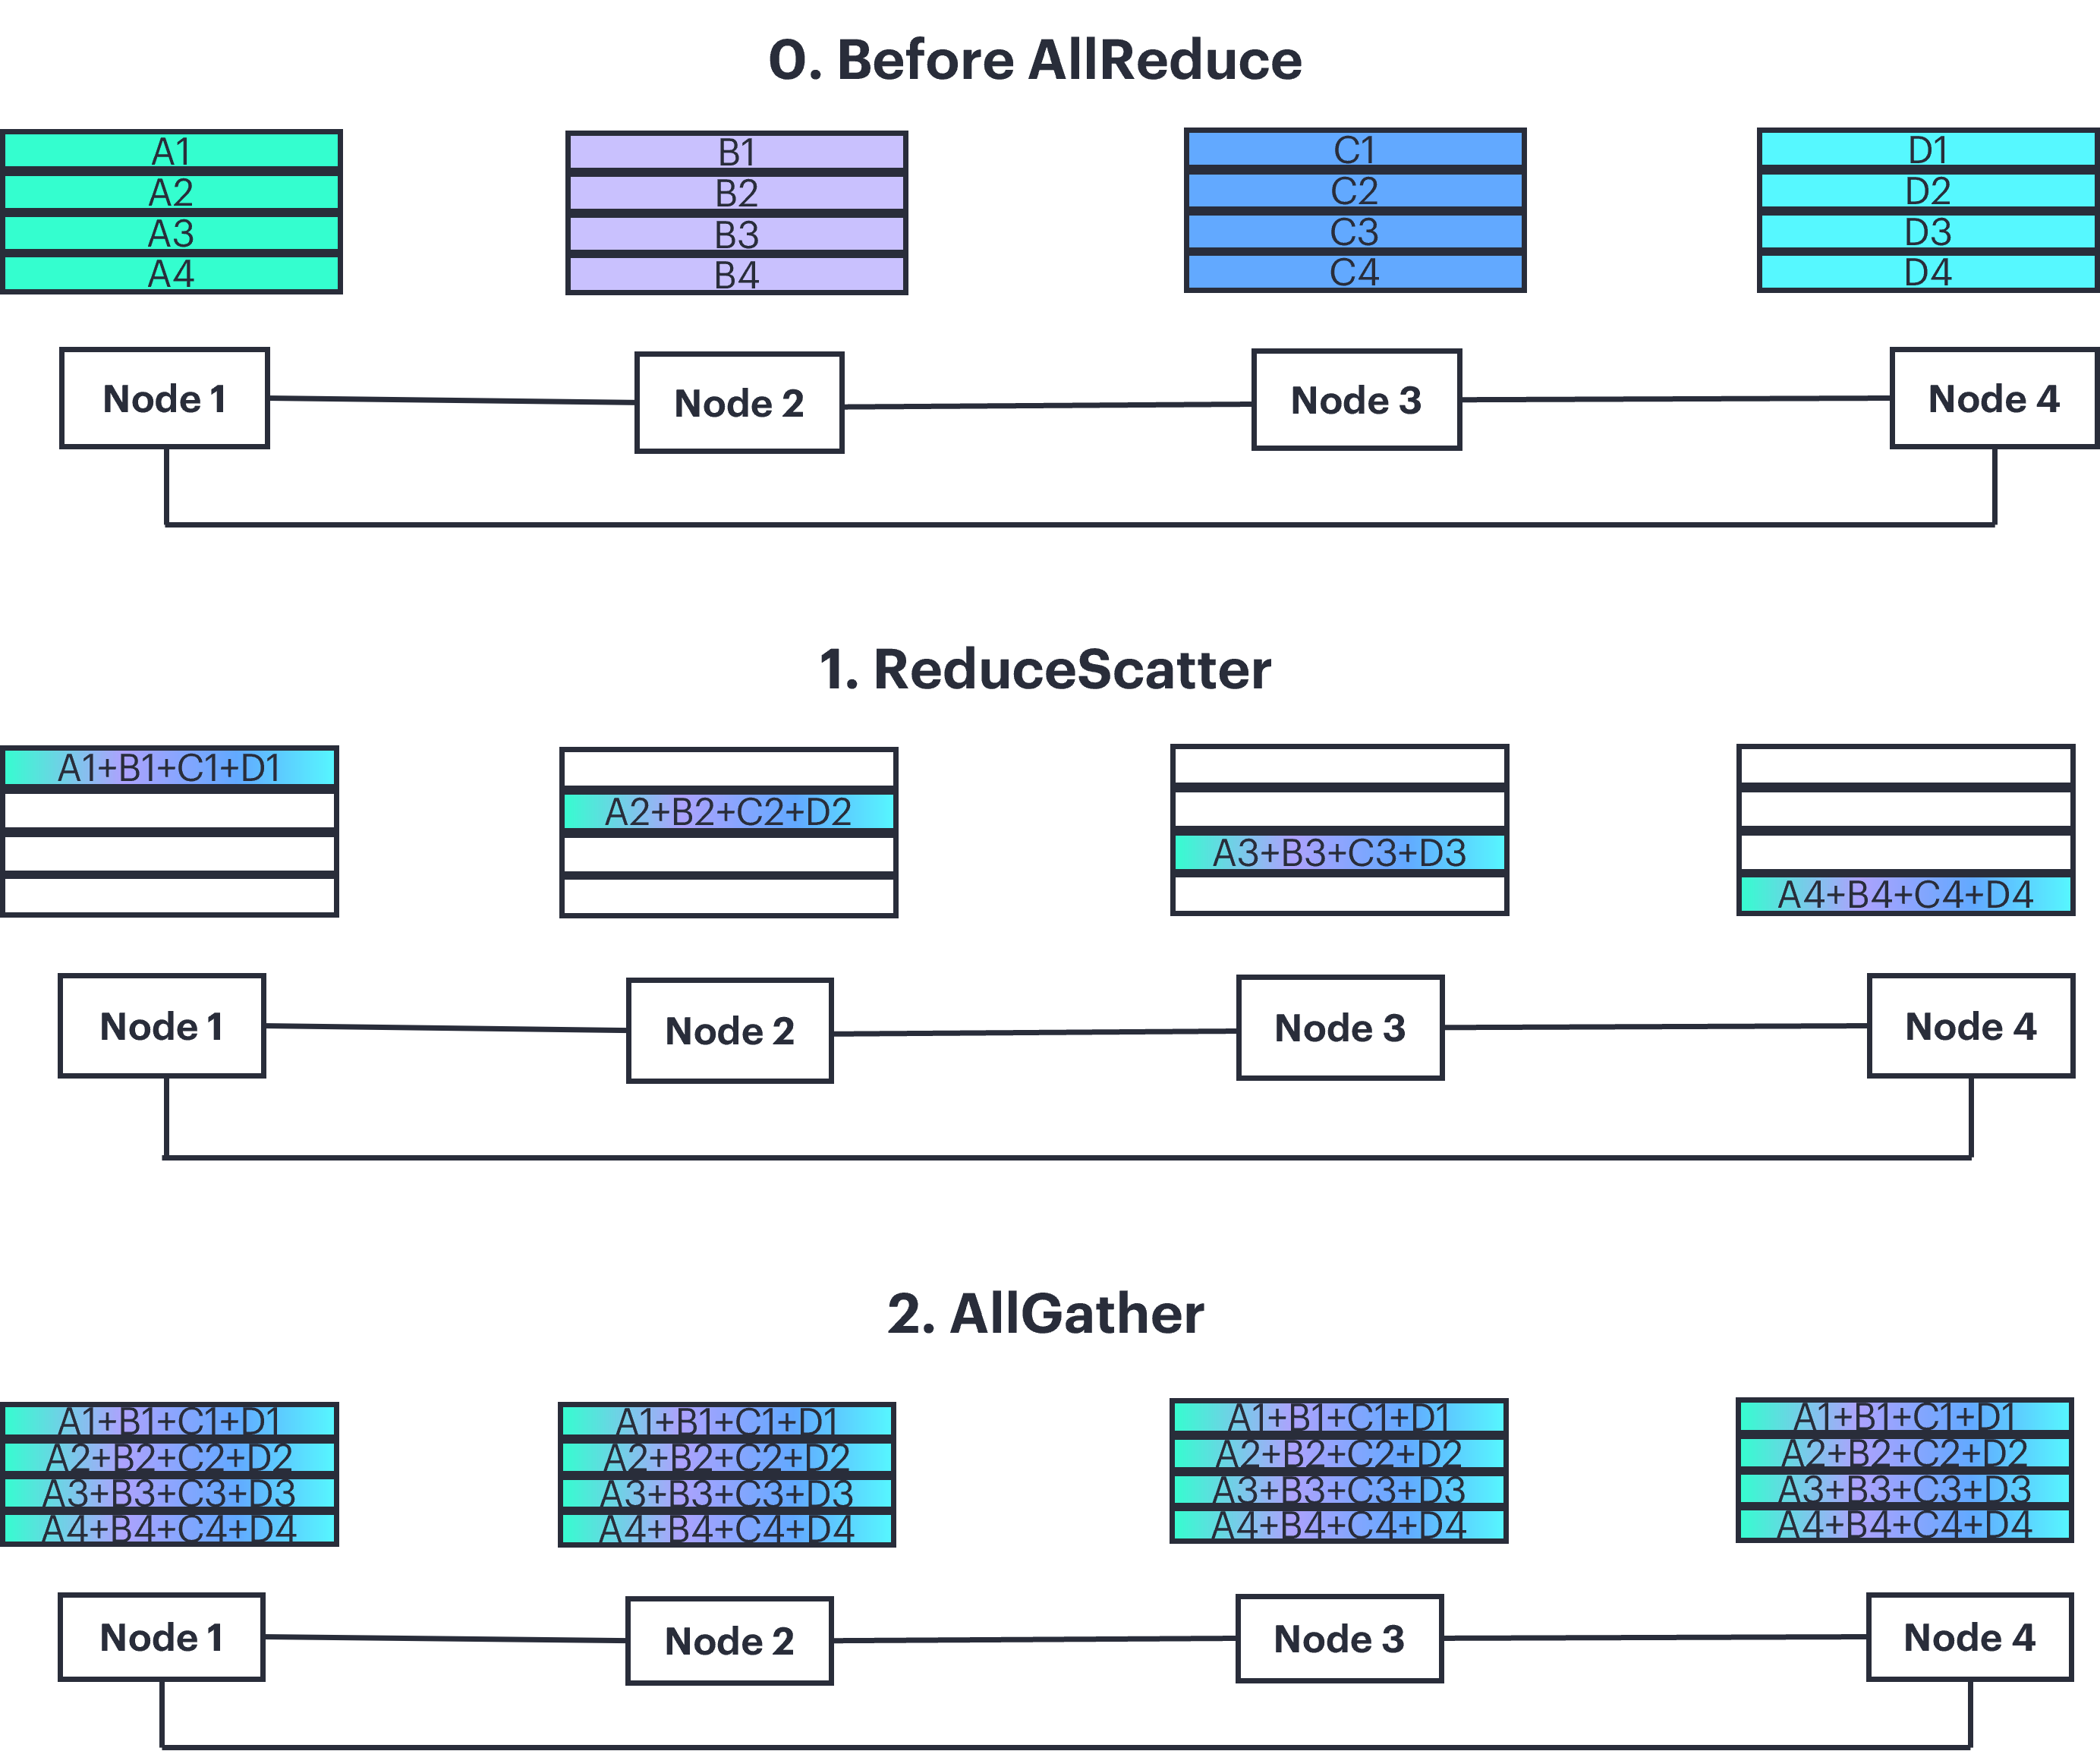
\includegraphics[width=0.9\linewidth]{collectives.png}
  \caption{All-Reduce}
  \label{fig:collectives}
\end{figure}

This collective can be used for $p$ nodes with each having a  $p$-sized vector of values. 
This example uses $p = 4$, four nodes with each having four parameters that the model gets trained on. 
Every node needs to know the number of $p$ and which index they have, meaning which parameter they are going to be responsible for. Also, this example uses a ring topology for easy visualization. The actual implementation can differ, in the following the theoretical background gets explained, more on that afterward.

In every iteration, the communication starts when all workers, here called nodes, are finished with their computation. Every Node has their four parameters stored.
The first step of the \textit{All-Reduce} is a \textit{Reduce-Scatter}, which itself involves two steps, a \textit{Scatter} and a \textit{Reduce}. \textit{Scatter} is the redistributive operation that shares every $i$-th parameter to the $i$-th node. With this, the first node receives all first parameters, the second all second ones and so on. 
\textit{Reduce} is the consolidative operation, that combines the received set of parameters to one single aggregation.
Together, they make every $i$-th node store one value in their $i$-th vector-place, combining the previous $i$-th values in every node's vector.

The second step is an \textit{All-Gather}, which is an advanced version of \textit{Gather}. That is an operation that is the reverse of \textit{Scatter}, as it combines every $i$-th nodes $i$-th value in one vector. \textit{All-Gather} expands this by a \textit{Broadcast}, which is the reverse of \textit{Reduce} and distributes the resulting vector to all nodes.
Afterward, the \textit{All-Reduce} is finished, and every node has a $p$-sized vector of the combined and shared values.

The used operations can be implemented  on top of various topologies, which influences how efficient the operation performs. In figure \ref{fig:topologies-logical}, common logical topologies are visualized. They can be for example a \textit{Mesh}, \textit{Tree}, or \textit{Ring}.

\begin{figure}[H]  % TODO make a visualization (that is wrongly the one for networks!)
  \centering
  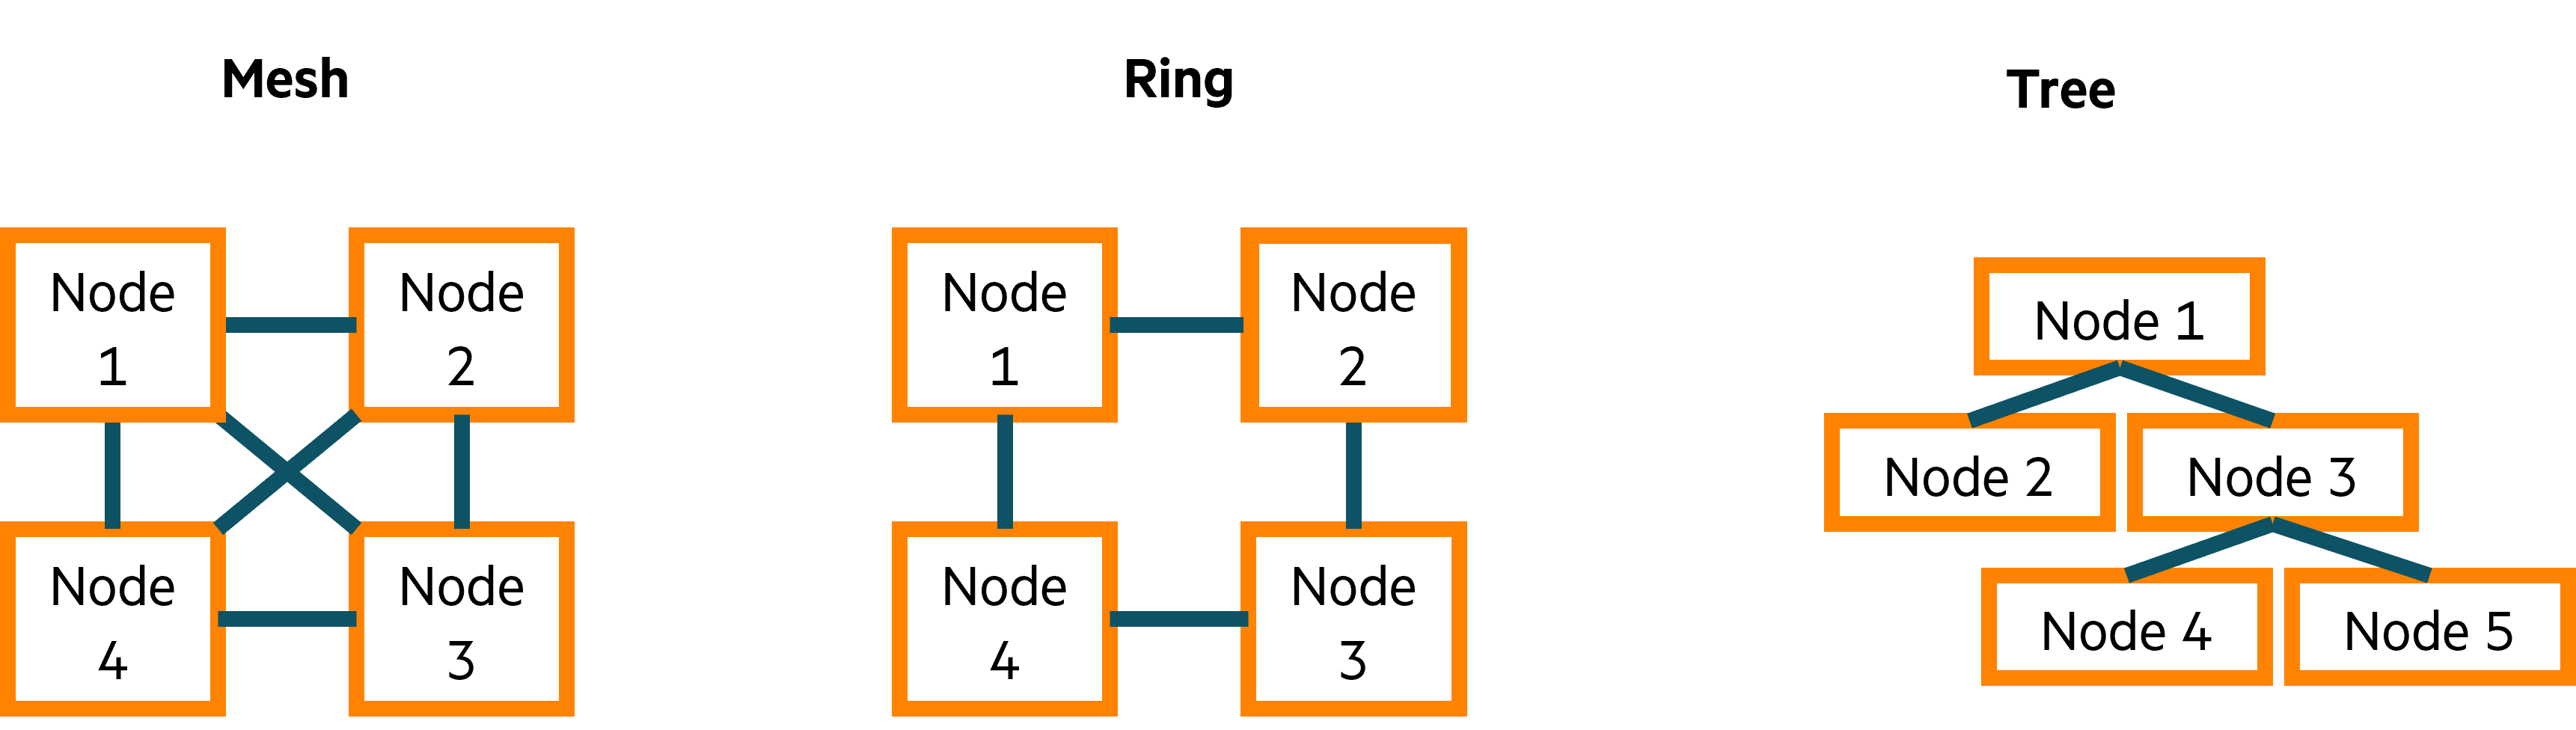
\includegraphics[width=1\linewidth]{topologies-logical.png}
  \caption{Logical Topologies}
  \label{fig:topologies-logical}
\end{figure}

Depending on the underlying physical topology, different logical topologies can be useful for the different collectives, as different complexities of bandwidths are relevant. Also, overlay topologies can be used to create virtual links to support exchanging data between unconnected nodes. % TODO check
Furthermore, topologies can be defined on multiple dimensions. Examples are a two-dimensional ring or a three-dimensional torus.


% Depending on the type of communication and 
% Another factor of \ac{DML} is the type of communication. 

% Algorithm
% While those topologies are showing different ways of centralization, they all more or less support synchronous as well as asynchronous communication. 

% Topologies

\subsubsection*{DML Challenges}
\label{sec:discussion}
% 4. Communication vs Computation, Parallelization strategy, extension ML to DML (maybe between section 1 and 2)
With many factors to consider, the \ac{DML} process allows a high range of configurations.
The first challenge is the communication overhead created when synchronizing shared parameters with workers that have different efficiency in their computations. 
Especially in centralized topologies with synchronized communication, workers waiting for others to finish should be avoided~\cite{sze_hardware_2017}. 
% \todo[inline]{Which topologies?} TODO
Additionally, when increasing computation allowance between communication times, a decrease of accuracy is likely to happen, as the model is trained less cohesively~\cite{yang_balancing_2025}.

Yang et al. claim that nowadays configurations of large \ac{DML} systems base on decentralized architectures with asynchronous communication~\cite{yang_balancing_2025}. 
% TODO add maybe more...
Challenges like those get solved by research and evaluation tests of many configurations. Such adn apporach needs to consider model accuracy, energy consumption, throughput and latency, and cost\cite{lee_model_2014}. To save resources and optimize configuration finding simulators can be used.

\section{ASTRA-Sim and Related Simulation Tools}

%% Simulation relevance
%%% Fault tolerance, heterogeneity, stragglers, energy efficiency
%%% Algorithms vs infrastructure interplay
%%% Simulation/benchmarking necessity (bridges into next section

% TODO write if time and space necessary

The most extensive publicly available \ac{DML} simulator with a focus on \ac{SW}/\ac{HW}-Co-Design is \ac{ASTRA-Sim}~\cite{rashidi_astra-sim_2020}.  
Its goal is to enable researchers to model and analyze configurations of \ac{DML}. It has a focus on hierarchical systems and communication for both intra- and inter-node-communication.
While there are many different versions of \ac{ASTRA-Sim} the following explanation focusses on \ac{ASTRA-Sim} 1.0 with an analytical backend. Explanations and comparison to other versions are provided in the subsection \ref{sec:comparison}.

% ASTRA-sim: 
% 1. Grundkonzept
\subsubsection*{ASTRA-Sim Approach and Implementation}
Generally \ac{ASTRA-Sim} consists of layers which enable users to configure and simulate specific input fields. The core of ASTRA-Sim features two parts. A workload layer that is used to specify the to be trained model, with expected layers of communication, and a system layer that can enable configure used collectives and scheduling policies.
\ac{ASTRA-Sim} is a network centered simulator, naturally an additional feature layer lets the user configure physical dependencies like topologies and bandwidths.
Initially, \ac{ASTRA-Sim} featured the existing Garnet network simulator \cite{agarwal_garnet_2009}. % TODO one sentence more

The workload layer uses an external computation model, like Scale Sim~\cite{samajdar_scale-sim_2019} to calculate each layers used \acp{GEMM}. Its inputs are based on the parallelization strategy \textit{(Data, Model, Hybrid)}, size of communication and structure of layers. 

The system layer implements collective operations dependent on logical topologies \textit{(All-Reduce, All-Gather, ...)}. Other configurable dependencies are the scheduling policy \textit{(\ac{LIFO}, \ac{FIFO})} and specifics such as the amount of splits of the dataset or \acp{LSQ}, which are the active chunks processed per dimension. This layer is able to simulate different phases in the communication, like multistage collectives and real-time differences between multiple dimensions.
% TODO introduce LIFO and FIFO bevore so it is in acronyms here...

The network layer simulates the hardware dependencies. The analytical version is able to consider configurations for multiple dimensions too. For each dimension a topology \textit{(Ring, Fully Connected, Switch)} with its amount of \acp{NPU} can be specified. The simulator includes latencies for links, routers and \acp{NIC} and bandwidths for links. The number of links is also important. Lastly the network layer can also simulate \ac{HBM}, with its latency, bandwidth and memory scale. 
% TODO introduce NICS before (i think i did, didnt I?) TODO AND introduce HBM!!

% A feature layer necessary for \ac{ASTRA-Sim} to work is a network layer. 
% three parts, called layers. They are separate simulators for workloads, system and the underlying network. 
Figure \ref{fig:astra-architecture} shows the original architecture with the Garnet network simulator. The different network backends are interchangeable as they all implement the same \etxtit{AstraNetworkAPI}.

\begin{figure}[H]
    \centering
    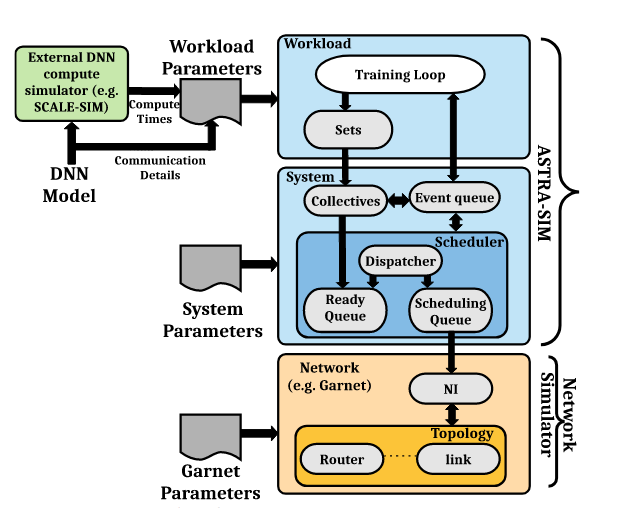
\includegraphics[width=0.6\textwidth]{astra-architecture.png}
    \caption{ASTRA-sim Architecture Overview, Official ASTRA-Sim 1.0 release~\cite{rashidi_astra-sim_2020}}
  \label{fig:astra-architecture}
\end{figure}

Each simulation iteration start with the initialization, where the user can specify their configurations. In the implementation this is separated by layer to a \ac{JSON} file for the network, a \ac{TXT} file for the system and a \ac{TXT} file for the workload. 
In the second step the workload gets produced. The loop produces sets of communication which again get separated into chunks for the processing.
In the next step the chunks get sorted into \acp{LSQ} and dispatched. This stream gets supervises and restarted if necessary. 
Next the final network simulation happens. In the analytical network the backend network gets simulated purely mathematically.
Lastly, \ac{ASTRA-Sim} exports its results into \ac{CSV} files. These show among other aspects the time of communication per layer, the distribution of computation vs communication and bottlenecks.

% \subsubsection*{Configurable Inputs}
% % 2. Network
% % 3. System
% % 4. Workload

\subsubsection*{Versions and Modifications of ASTRA-Sim}
\label{sec:comparison}
Its initial release in 2020 includes a Garnet network. It was expanded later by an analytical network simulation. While Garnet is cycle accurate, so it simulates clock and packets in detail, the analytical network is based on mathematical approximate models. Therefore, the analytical model is slightly inaccurate, as it is for example not congestion aware, but it is more scalable than the garnet network.

% 5. 2.0 & more extensions
In 2023 a second version of \ac{ASTRA-Sim} was released~\cite{won_astra-sim20_2023}. It addresses the need for a higher scalable simulator, as deep learning models grew. % TODO is documentation the right word?

The loop is similar, with a few changes and extensions.
First, the workload layer process. This workload layer was replaced with a chakra traced based workload layer. That is a graph based workload documentation~\cite{sridharan_chakra_2023}.
So, it replaces the previous static trainings loop with a dynamic one based on \acp{ET}. An \ac{ET} is a graph that reproduces a real \ac{ML} training process. Each of its nodes represents either a \ac{GEMM}, an access of memory or a collective communication. They can for example be extracted form frameworks such as PyTorch and converted to Chakra \acp{ET}.
This workload layer supports more specific parallelization strategies than the 1.0 version \textit{(Pipeline, Hybrid-Parallel, ...)}. % TODO check if that makes sense, because hybrid was existing before
This represents a more realistic model of parallelization, as the \acp{NPU} are capable of executing varying operations. 
After the \ac{ET} is read and distributed on configures \acp{NPU}, each gets its own graph to simulate. Time spend on the computation, communication and usage of storage get collected. These use other layers information.

The system layer still manages the collective operations, depending on topoogies and scheduling strategies. A relevant difference to 1.0 is input got reduced to the only necessary parameters, ones reflected by chakra traces were crossed out. As a result it only features a topology, number of \acp{NPU}, internal bandwidth and internal latency. % TODO i think that is not interelly true.
The idea is to completely abandon the inputs and retrieve them from chakra \ac{ET} too.

% Network layer replacement
For network simulation the network layer was used, and the two existing implementations were revised and additional backends added. 
The analytical backend is still implemented as a scalable and fast approximate network simulator, but the Garnet backend was abandoned.  
Now instead the \ac{NS-3}~\cite{riley_ns-3_2010} and the \ac{HTSim}~\cite{besta_towards_2021} backend can be used for the network simulation. 
The \ac{NS-3} is a well established network simulator, that includes realistic network conditions with congestion and routing, which makes it suitable for simulation that needs to be very accurate and realistic. \ac{HTSim} rather focusses on the integration of Ultra Ethernet, an alternative to the standard \ac{TCP}. It is more lightweight and an alternative to the \ac{NS-3} that includes view of network traffic as flows rather than individual packets, which is especially relevant for \ac{DML} setups.
Both are more accurate than the analytical model. % (which reaches up to 95\% accuracy~\cite{.})
% HTSim: Ultra Ethernet -> protocolle welche tcp ersetzen für workloads in HPC, AI und storage
% INFINIBAND UND SLINGSHOT (kein ethernet) TODO they both need to presented and earlier

The 2.0 version also includes a new layer, called memory layer. It is connected via an own memory \ac{API}. This models the \ac{HBM} previously managed by the system layer. It supports disaggregated memory architectures and realistic pipelines transfers with their according bandwidths, latencies and topologies. That way \ac{ASTRA-Sim} is able to compare these different known memory architectures depending on underlying \ac{DML} configurations.

In general, \ac{ASTRA-Sim} 2.0 is more flexible that 1.0, by allowing many more configurations and realistic workloads. Its disadvantage is, that it is still being developed and changes are introduced. For a stable simulation 1.0 is the better choice, but in the future and for current research 2.0 will be more relevant.


\subsubsection*{Comparison to Further Simulation Tools}
% Weitere Tools: NS-3, MLPerf, SimGrid: Use cases & why it was not considered here

A specialty of \ac{ASTRA-Sim} is that it supports hierarchical topologies, so it can model asymmetrical bandwidths. Also, it allows a differentiation between logical and physical topologies. This is especially relevant for research contexts.
Additionally, it is easily extendable as layers can be exchanged and new factors such as new topologies or strategies can easily be added.

% It is the only ...

% TODO write if necessary


% \begin{table}[H]
%     \centering
%     \caption{Feature comparison of simulation tools}
%     \begin{tabular}{lccc}
%         \toprule
%         Tool      & Simulation Type & UI Support & Notable Features  \\
%         \midrule
%         ASTRA-sim & Network-level   & CLI only   & HPC-focused       \\
%         SimGrid   & System-level    & Minimal UI & Flexible modeling \\
%         NS-3      & Packet-level    & CLI/GUI    & Networking focus  \\
%         MLPerf    & Benchmarking    & Web UI     & ML performance    \\
%         \bottomrule
%     \end{tabular}
% \end{table}


\section{User Interface Design for Scientific Tools}
% Accessibility, UI patterns, visualization  ==> I HAVE TO DO LITERATURE REVIEW FIRST!!!!!
% Human-Machine Interaction

% \subsubsection*{Role of UI in Scientific Tools}
% CLI vs GUI in research context
% Define UI, UX, HCI

Research tools in computer science are mostly based on \acp{CLI}. Including \acp{GUI} can increase use cases and amount of usage~\cite{sampath_accessibility_2021}.
While \ac{UI} refers to the visual and interactive design of a digital product, \ac{UX} refers to the entire experience users go through when using digital tool. Both areas are highly interconnected and central for the users' satisfaction with a digital product~\cite{hamidli_introduction_2023}. % for developing a useable interface for digital tools.
The study of \ac{UI} and \ac{UX} is \ac{HCI}, which in return gives it a scientific base. 
In the following, design principles of \acp{UI} in general and in this projects specific context get explained and the current state of the art presented.  % TODO passe an nachdem das kapitel geschrieben ist


\subsubsection*{Human-Computer Interaction Foundations}
\ac{HCI} is an interdisciplinary area that deals with the design, evaluation and implementation of interactive computer systems~\cite{sinha_human_2010}. Its goal is to improve these systems in their functionality and usability. 
Specific goals also include methods for designing and implementing user-friendly \acp{UI} as well as criteria for evaluating and comparing interfaces. \ac{HCI} also focusses on the development of new interaction techniques and models to human machine interactions. 

This discipline was relevant from the moment on the first electronic computer in 1946 was used, called the \ac{ENIAC}~\cite{goldstine_electronic_1996}, which was used for computation of military firing tables. Later, with the development of \acp{GUI}, the internet and a wide base of useable tools, \ac{HCI} became an important field, also relevant for website design.

\ac{HCI} claims that machines are worthless until they are properly useable. Two main aspects are the functionality and usability of machines.
Functionality refers to the set of services a program provides. This value becomes only value if it is useable efficiency.
Usability is the extent of which the system helps the users to activate their goals when using the machine. It depends on the needs of the target user group.
Generally, in \ac{HCI} a system is only considered qualitative, if functionality and usability are balanced.

% Cognitive Load
One important sub category of \ac{HCI} is cognitive load. Kosch et al.~\cite{kosch_survey_2023} present its characteristics and measurements in the following way. 
Defining cognitive workload is a challenge, it describes the amount of complexity the human brain gets presented with when executing tasks. In the field of website \ac{GUI} design this can be transferred as the complexity of brain processes a user goes through to navigate the website. Naturally, they should be minimized to ensure the least possible complexity when using the website. % TODO erwähne in chapter 3 die idee von einer NLP input, weil dass hier dann relevant wird.
Because digital systems are getting increasingly more complex, measurements of cognitive workloads gets increasingly more difficult. They present metrics such as questionnaires, which are very subjective, physiological sensors which are very objective or presented behavior, like the users mouse activity.
With those evaluations different layouts or navigation structures can be tested and compared. 
% TODO write more --> congitive load relative to other layouts etc

% Principles of usability
% Viuzualization

% Feedback loops
Another important sub-field of \ac{HCI} are feedback loops. Feedback is the direct response of a system to a users action and is central for users, especially when they interact with computers in the wrong way. %, but also important evidence for the user to satisfy thair expctations
In \ac{GUI} design for example when entering values in a form or uploading files that are not meeting specific criteria, it needs to be made sure that users understand what went wrong and to give them feedback to reduce the possibility of this problem occurring again. No feedback, delayed feedback and wrong feedback can make the user feel frustrated and unable to take full advantage of functionalities.
Pérez-Quiñones and Sibert present a foundational study on the feedback model based on the linguistic theory of \ac{SOU}~\cite{perez-quinones_collaborative_1996}.
That is a model explaining which state humans think they are in during a conversation, based on expectations they have when communicating with each other.
Instead of seeing communication as ping-pong iterations between two participants, here it is viewed as collaborative process based on Clark et Al.~\cite{clark_grounding_1991}. Basically, it includes four states a listener can be in after a speaker send a message. 
% For example when a user input data into a form the computer can differentiate between not having received the input, not having understood the input, ...
This original concept from the linguistic area was applied onto the \ac{HCI} area.
The resulting five \ac{SSOU} represent states needed in communication between humans and computers to match the humans expectations. The stages are:

\begin{flushleft}
1.~The system is ready to receive inputs, \\
2.~The user entered an input and the system processes that, \\
3.~The result gets reported by the system, \\
4.~The system ignores the input, \\
5.~The system stores the inputs for a later processing. 
\end{flushleft}

For every stage the computer needs to provide specific feedback, so the user feels informed, and unnecessary interactions can be reduced. 

% TODO in chapter 3 erwähne dass der fake sinner auf processing stage hindeutet AUCH: hpe grommet design vieles dementsprechend, buttons hervorgehoben etc


\subsubsection*{UI/UX Best Practices and Evaluation Metrics}
% Nielsen’s usability heuristics
% Quantitative: task completion time, error rates, learning curve.
% Qualitative: SUS (System Usability Scale), UEQ (User Experience Questionnaire).
% Research-specific: reproducibility of workflows, error prevention in simulation setup.
% mass user testing vs expert testing in my context
% Mention: when a UI targets multiple groups, evaluation must consider different user personas (e.g., researchers vs. business users).


% Personas DELETED BECAUSE: I do not have a dataset that i can base a persona on.
One aspect that needs to be considered is the difference that target user groups bring with them. One technique to characterize user groups is by using personas~\cite{billestrup_persona_2014}. Using personas is supposed to help developers understand expectations, goals and contexts of users, to optimize the end product for the user.
That way the user is central for the design process and can specifically be targeted. How efficient personas are depends on the quality of data it is based on and the depth of them.
There are many possible strategies of building personas based on existing datasets. If there is no dataset available, an approach including expert interviews, existing knowledge and assumptions have to be used~\cite{pruitt_personas_2003}. 
Each personas specification should include information such as daily routines, goals, fears, attitudes, technology behaviour, demographics, and existing knowledge.
Personas can be used to design specific usability tests or specifications of necessary functionality. 
Combined with \ac{HCI} it can be used to evaluate the necessity of certain aspects such as the extent of necessary feedback.

% Non expert vs Expert users
One classification that could be made for users is whether they are experts or non-experts in the field of the website. This is especially important for scientific tools, as they deal with specific areas that are not relevant in daily life of most people.
An expert in the field of usability and \ac{HCI} is Nielsen, that states that intuitiveness is central for website usage for novice users~\cite{nielsen_differences_2006}. Even though his post was publicized in 2000, it still holds relevance today, but has to be regarded with conciseness. 
He states that the interface has to be differentiated between expert and novice users. While non-experts should be getting training-wheel designs to get guidance of usage, experts should get interfaces that provide a powerful tool set.
Also, the development from novices to experts can be supported but need to be observed with usability tests.

% Practical evaluation metrics
A recent approach of methodically revising and restructuring \ac{UI} recommendations was done by Diehl et Al in 2022\cite{diehl_defining_2022}. The method included expert interviews and a content analysis with a revalidation of an expert group.
The resulting $69$ general recommendations can be divided into $12$ categories. These are feedback, recognition, flexibility, customization, consistency, error handling, help, accessibility, navigation, privacy, visual design and emotional design. The entire list can be found in the appendix~\ref{appendix:A}.
The recommendations are closely connected to presented \ac{HCI} approaches. Mentionable recommendations for instance also include that systems should enable users to easily recognize user functions (recognition, rule 3), it should ensure consistency in appearance (consistency, rule 1), it may concentrate the information mainly in the center of the screen (visual, rule 2), and it should provide the options and information in a logical sequence (navigation, rule 1). Further relevant rules are presented in chapter \ref{chap:design}.

% TODO add evaluation metrics for things measured in chapter 5

% \subsubsection*{UI and UX in Scientific and Simulation Tools}
% Specific challenges
% Inwiefern exsiting Simulators have UIs
% Add: discuss how tools like TensorBoard and Jupyter already cross the boundary between research and broader communication (used by data scientists and ML engineers, not just simulator developers)
% Position your contribution: few simulators have UIs that also support non-technical exploration



% Prepare the ground for your own UI: “While most UIs in scientific simulators focus exclusively on expert users, our work considers broader accessibility, enabling stakeholders outside research — such as sales — to interact meaningfully with the simulator results.”














% TIPS VON CHATTI
% Be selective: Don’t include everything—focus on what’s most relevant
% Synthesize, don’t summarize: Show connections, contradictions, and trends
% Use visuals: Diagrams, tables, or concept maps can clarify complex relationships
% End with a gap: Clearly state what’s missing in the literature and how your work fills it